\subsection{Appearance of Period-adding structures}
\label{sec:add.change.appa}

In this section we will explore the appearance of the period-adding structures in between the chains of the same period.
This happens at the horizontal boundaries between ``type A'' parameter regions of different chains, as well as at the vertical boundaries.
We will first take care of the horizontal period-adding structures and then move on to the vertical period-adding structures.

\subsubsection{Horizontal Period-adding Structures}
\label{sec:add.change.appa.hor}

In \Cref{fig:add.change.regions.1}, the ``type A'' parameter regions $P^{20}_3$ and $P^{18}_3$, as well as $P^{22}_4$ and $P^{20}_4$ overlap.
This changes in \Cref{fig:add.change.regions.2}.
Here only the ``type A'' parameter regions $P^{20}_3$ and $P^{18}_3$ overlap, the parameter regions $P^{22}_4$ and $P^{20}_4$ stopped overlapping.
Instead, in the space between the two ``type A'' parameter region there are now two asymmetric coexisting twin cycles $\Cycle{\A^8\B^3\C^8\D^2}$ and $\Cycle{\A^8\B^2\C^8\D^3}$.
Those cycles are \textbf{not} ``type B'' cycles, because they only differ in the number of points on the branches $f_\B$ and $f_\D$.
Instead, we will call them hybrid cycles and ``type B'' cycles are a special case of hybrid cycles.
The notation $\left[P^{22}_4 \mid P^{20}_4\right]$ used in the diagrams was introduced in \Cref{sec:add.change} and is formally defined later in \Cref{sec:add.add.halved}.
Later in \Cref{fig:add.change.regions.4}, the ``type A'' parameter regions $P^{20}_3$ and $P^{18}_3$ also stop overlapping.
In between, there are also hybrid cycles, $\Cycle{\A^7\B^3\C^6\D^3}$ and $\Cycle{\A^6\B^3\C^7\D^3}$.
This parameter region is therefore labeled $\left[P^{20}_3 \mid P^{18}_3\right]$.

In between \Cref{fig:add.change.regions.2,fig:add.change.regions.3}, the ``type A'' parameter regions $P^{22}_4$ and $P^{20}_4$ don't stop overlapping completely.
Instead, they only stop overlapping on the left side of their shared boundaries and the rest is not pictured in these diagrams.
\Cref{fig:add.change.appa.hor.regions} shows better what happens to this overlapping region between \Cref{fig:add.change.regions.1,fig:add.change.regions.4}.
We also have a codimension-2 point that moves right as was the case in \Cref{sec:add.change.disb}.

\todo{Regions: labels wrong}
\todo{Cobwebs: enhance borders, replace (c), wrong pic}
\begin{figure}
	\centering
	\subfloat[Regions]{
		\includegraphics[width=.3 \textwidth]{62_MinimalRepr_Adding/2D_Regions_2.8_add_hor/Manual/result.png}
		\label{fig:add.change.appa.hor.regions}
	}
	\subfloat[At point $A$]{
		\includegraphics[width=.3 \textwidth]{62_MinimalRepr_Adding/Cob_2.8_add_hor_A/Manual/result.png}
		\label{fig:add.change.appa.hor.cob.A}
	}
	\subfloat[At point $B$]{
		\includegraphics[width=.3 \textwidth]{62_MinimalRepr_Adding/Cob_2.8_add_hor_A/Manual/result.png}
		\label{fig:add.change.appa.hor.cob.B}
	}
	\caption{Appearance of the horizontal period-adding cascade}
\end{figure}

We know from \Cref{sec:arch.bif.sum} that the \gls{bcb} at the upper boundary of the ``type A'' parameter region $P^{22}_4$ is $\BCB_{d_1, d_3}^{\underline{\A}^7\B^4\underline{\C}^7\D^4}$.
And the \gls{bcb} at the lower boundary of the ``type A'' parameter region $P^{20}_4$ is $\BCB_{d_1, d_3}^{\A^6\underline{\B}^4\C^6\underline{\D}^4}$.
Both these \glspl{bcb} are at the upper and lower boundaries of the overlapping region $P^{22}_4 \cup P^{20}_4$.
At the codimension-2 point, both these \glspl{bcb} happen at the same time and both cycles vanish.
We can see in \Cref{fig:add.change.appa.hor.cob.A} that the ``type A'' cycles are very close to the borders $d_1$ and $d_3$, respectively.

This codimension-2 point moves right with higher values for $b_L$ along our line.
As soon as the codimension-2 point crosses the right boundary of either the ``type A'' parameter region $P^{22}_4$ or $P^{20}_4$, the overlapping parameter region $P^{22}_4 \cup P^{20}_4$ ceases to exist.
Instead, there is space between the two ``type A'' parameter regions where there are now two hybrid cycles and period-adding between the hybrid cycles and either ``type A'' parameter region.

\todo{Labels for bifurcations missing underline}
\begin{figure}
	\centering
	\includegraphics[width=.7 \textwidth]{62_MinimalRepr_Adding/1D_Bif_2.8_add_hor_AU/Manual/result.png}
	\caption{Bifurcation diagram at the upper boundary of $\left[P^{22}_4 \mid P^{20}_4\right]$}
	\label{fig:add.change.appa.hor.bif}
\end{figure}

We assume that the \glspl{bcb} bounding the parameter regions with hybrid cycles follow the same rules as the \glspl{bcb} bounding the ``type B'' parameter regions.
\Cref{fig:add.change.appa.hor.bif} confirms this for the upper boundary.
So it is bounded at the top by the \glspl{bcb} $\BCB_{d_1}^{\underline{\A}^7\B^4\C^6\D^4}$ and $\BCB_{d_3}^{\A^6\B^4\underline{\C}^7\D^4}$.
And bounded at the bottom by the \glspl{bcb} $\BCB_{d_3}^{\A^7\B^4\C^6\underline{\D}^4}$ and $\BCB_{d_1}^{\underline{\A}^6\B^4\C^7\D^4}$.
At the codimension-2 point, both \glspl{bcb} $\BCB_{d_1}^{\underline{\A}^7\B^4\C^6\D^4}$ and $\BCB_{d_3}^{\A^7\B^4\C^6\underline{\D}^4}$ happen to the cycle $\Cycle{\A^7\B^4\C^6\D^4}$ at the same time and it vanishes.
Because of the symmetry, the \glspl{bcb} $\BCB_{d_3}^{\A^6\B^4\underline{\C}^7\D^4}$ and $\BCB_{d_1}^{\A^6\underline{\B}^4\C^7\D^4}$ happen to the cycle $\Cycle{\A^6\B^4\C^7\D^4}$ at the same time and it vanishes also.

\todo{also confirmed by cobweb with enhanced cycles at borders}

How this overlapping parameter regions disappears is similar to how the overlapping parameter region appears in \Cref{sec:add.change.disb}.
There, the codimension-2 point removes the ``type B'' parameter region and opens the overlapping parameter region.
Here, the codimension-2 point removes the overlapping parameter region and opens the parameter region with hybrid cycles, which behave very similar to ``type B'' cycles.

\subsubsection{Vertical Period-adding Structures}
\label{sec:add.change.appa.vert}

For the vertical period-adding structures, we could not find a codimension-2 point like for \Cref{sec:add.change.disb,sec:add.change.appa.hor}.
In \Crefrange{fig:add.change.regions.1}{fig:add.change.regions.2}, the parameter regions $P^{20}_3$ and $P^{22}_4$, as well as $P^{18}_3$ and $P^{20}_4$ overlap.
The appearance of the parameter region $\left[P^{20}_3 \mid P^{22}_4\right]$ in between $P^{20}_3$ and $P^{22}_4$ seems to happen at the same time as the appearance of the hybrid parameter region $\left[P^{18}_3 \mid P^{20}_4\right]$ in between $P^{18}_3$ and $P^{20}_4$.
At some parameter values on the line between \Cref{fig:add.change.regions.3,fig:add.change.regions.4}.
And with these hybrid parameter regions the vertical period-adding-like structures between them and the neighboring ``type A'' parameter regions.

\Cref{fig:add.change.appb.regions.A,fig:add.change.appb.regions.B} show this transition again for the parameter regions $P^{20}_3$ and $P^{22}_4$.
The transition might be similar to the previous \Cref{sec:add.change.disb,sec:add.change.appa.hor} with a codimension-2 point that moves up or down, or it could happen at once with the left boundary of $P^{22}_4$ and the right boundary of $P^{20}_3$ being aligned perfectly for some parameter values of $a_L$ and $b_L$ on the line given by \Cref{equ:add.change.paramline}.

\todo{Regions: labels wrong}
\todo{Cobwebs: replace (c) and enhance cycles at borders}
\begin{figure}
	\centering
	\subfloat[Regions scan before period-adding\\at $a_L = 2.8, b_L = -0.1$]{
		\includegraphics[width=.4 \textwidth]{62_MinimalRepr_Adding/2D_Regions_2.8_add_vert/Manual/result.png}
		\label{fig:add.change.appa.vert.regions.A}
	}
	\subfloat[Regions with period-adding\\at $a_L = 2.65, b_L = -0.05$]{
		\includegraphics[width=.4 \textwidth]{62_MinimalRepr_Adding/2D_Regions_2.65_add_vert/Manual/result.png}
		\label{fig:add.change.appa.vert.regions.B}
	} \\
	\subfloat[At point $A$]{
		\includegraphics[width=.4 \textwidth]{62_MinimalRepr_Adding/Cob_2.8_add_vert_A/Manual/result.png}
		\label{fig:add.change.appa.vert.cobweb.A}
	}
	\subfloat[At point $B$]{
		\includegraphics[width=.4 \textwidth]{62_MinimalRepr_Adding/Cob_2.65_add_vert_B/Manual/result.png}
		\label{fig:add.change.appa.vert.cobweb.B}
	}
	\caption{Appearance of the vertical period-adding cascade}
\end{figure}

\Cref{fig:add.change.appa.vert.cobweb.A} shows the coexistence of the two coexisting ``type A'' cycles while the ``type A'' parameter regions still overlap.
\Cref{fig:add.change.appa.vert.cobweb.B} shows the coexistence of the two coexisting hybrid cycles in the newly created parameter region $\left[P^{20}_3 \mid P^{22}_4\right]$.

\begin{figure}
	\centering
	\includegraphics[width=.7 \textwidth]{62_MinimalRepr_Adding/1D_Bif_2.65_add_vert_BR/Manual/result.png}
	\caption{Bifurcation diagram of the right boundary of $P_{10}^3 \oplus P_{11}^4$}
	\label{fig:add.appa.vert.bif}
\end{figure}

\todo{old:}

\todo{odd number of splits => no neg slope needed for asymmetry. odd number => needed (reorders cycles)}
